\chapter*{Acerca del autor}
\label{chap:biografia}


\begin{figure}[H]
\centering
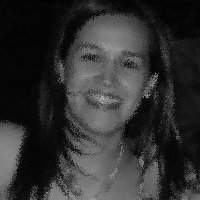
\includegraphics[width=4cm,keepaspectratio=true,clip=true]
{Figures/Biografia/Foto.jpg}\\
\label{Fig:Foto}.
\end{figure}

\begin{center}
\noindent \large \textbf{\textit{Romina Solorza}}\\
\end{center}


Licenciada en Geografía graduada de la Universidad Nacional del Comahue en 2008. Su tesis de grado se denominó “Estudio de degradación de tierras a partir de análisis fisiográfico y aplicación de técnicas de teledetección. Cuenca del río Guañacos. Provincia del Neuquén”. Fue becada en 2009 para realizar una especialización en el Laboratorio Aereo di Riprese Ambientali (LARA) en Roma, Italia. En 2010 fue becada para realizar sus estudios de posgrado en el Instituto de Altos Estudios “Mario Gulich” dependiente de la Comisión Nacional de Actividades Espaciales y de la Universidad Nacional de Córdoba para obtener el diploma de Magister en Aplicaciones Espaciales para Alerta y Respuesta Temprana a Emergencias. 

Su especialidad se orienta al procesamiento de imágenes satelitales ópticas y particularmente de radar (SAR). Ha trabajado en la gestión e integración de datos espaciales en SIG para estudios del ambiente, la hidrología y la actividad hidrocarburífera. Se desempeñó en distintos organismos, tanto públicos como privados, en tareas de análisis SIG y sensores remotos. Integró equipos técnicos en proyectos de planificación territorial y ambiental tanto en la provincia de Neuquén, como en Río Negro y Córdoba. Ha participado en proyectos de investigación en la Universidad Nacional del Comahue así como también en la CONAE y en el Instituto de Sensoramiento Remoto Aplicado de la Academia Europea (EURAC) en Bolzano, Italia.